\chapter{EXPERIENCE}

\begin{multicols}{2}

\index{Experience}Experience is a measure of the characters' improvement.  The GM is in charge of calculating experience points.  Experience is added up and divided evenly among all surviving players at the end of a session or adventure.  Dead characters or recently resurrected characters should receive experience for events that happened up to their death.  When a character gains enough experience to level up, they gain all the benefits of their new level.  Experience points (XP) can be assigned for anything requiring skill to overcome.  While experience can be assigned for devising a good plan to escape captors, it's best calculated through overcoming encounters and completing story related goals.

Overcoming encounters involves coming out the victor in a dangerous situation.  This is a broad ruling that can apply to many scenarios, but as a rule, it requires the characters to be in danger (or to perceive that they are in danger).  Defeating a band of monsters is overcoming an encounter.  Navigating through or disabling a trap, successfully evading a pursuing band of orcs, or convincing a gang of bandits not to attack passing caravans are other examples.  Setting off a trap using a rock from afar, however, is not, as the characters aren't in any risk of danger.  If they accidentally trigger a rolling rock that chases them through a trap, then they're suddenly pitted with an exceptionally tough encounter and should receive proportionately more experience points if they survive it.

Calculating experience for defeating enemies is based on their hit dice.  Opponents with special abilities or strengths are considered to have higher HD for the purpose of calculating experience points.  Monsters use d8 hit dice and a number following the HD is a modifier to their hit points (for example 1~+~1 means roll 1d8 then add 1).  This system can also be used to calculate experience gained for traps or deadly situations.  If a trap is sufficient to kill the average 7\textsuperscript{th} level character, then it should be considered a 7 HD creature for the purpose of earning experience.

\subsection{STORY RELATED EXPERIENCE}

Story related experience points are awarded whenever a prominent goal is completed.  As a general rule, story related experience points should never exceed the total experience awarded for overcoming encounters up to the completion of the goal.  Characters may also set personal goals for themselves. These goals should be sufficiently dangerous to warrant the awarding of experience points, and everyone who participates should earn a fair share.

\noindent
\begin{minipage}{\columnwidth}

\captionof{table}{Creature Experience Awards}\label{creaturexp}
\noindent
\begin{tabular}{|p{.3\columnwidth}|p{.6\columnwidth}|}
\hline
HD or Level		& XP Value \\
\hline\hline
\rowcolor[gray]{.9}Less than 1~$-$~1	& 7 \\
1~$-$~1 to 1		& 15 \\
\rowcolor[gray]{.9}1~+~1 to 2		& 35 \\
2~+~1 to 3		& 65 \\
\rowcolor[gray]{.9}3~+~1 to 4		& 120 \\
4~+~1 to 5		& 175 \\
\rowcolor[gray]{.9}5~+~1 to 6		& 270 \\
6~+~1 to 7		& 420 \\
\rowcolor[gray]{.9}7~+~1 to 8		& 650 \\
8~+~1 to 9		& 975 \\
\rowcolor[gray]{.9}9~+~1 to 10+	& 1,400 \\
11 to 12+		& 2,000 \\
\rowcolor[gray]{.9}13+				& 3,000~+~1,000 per HD over 13 \\
\hline
\end{tabular}

\end{minipage}

\noindent
\begin{minipage}{\columnwidth}

\captionof{table}{Hit Dice Value Modifiers}\label{hdvaluemods}
\noindent
\begin{tabular}{|p{.8\columnwidth}|p{.1\columnwidth}|}
\hline
Ability			& HD Mod* \\
\hline\hline
\rowcolor[gray]{.9}AC 0 or lower	& +1 \\
Blood drain		& +1 \\
\rowcolor[gray]{.9}Breath weapon	& +2 \\
Causes disease	& +1 \\
\rowcolor[gray]{.9}Energy drain	& +3 \\
Flying			& +1 \\
\rowcolor[gray]{.9}4+ attacks per round	& +1 \\
Above average HP		& +1 \\
\rowcolor[gray]{.9}High intelligence		& +1 \\
Hurt only by magic/silver	& +1 \\
\rowcolor[gray]{.9}Spell immunity			& +1 \\
Weapon immunity including $^1$/$_2$ damage	& +1 \\
\rowcolor[gray]{.9}Invisible at will		& +1 \\
Up to level 2 spells	& +1 \\
\rowcolor[gray]{.9}Level 3 or greater spells (not cumulative with above bonus)		& +2 \\
Magic resistance		& +2 \\
\rowcolor[gray]{.9}Missile weapons			& +1 \\
Multiple attacks causing 30+ points of damage	& +2 \\
\rowcolor[gray]{.9}Paralysis				& +2 \\
Petrification			& +3 \\
\rowcolor[gray]{.9}Poison					& +2 \\
Wields magical items	& +1 \\
\rowcolor[gray]{.9}Regeneration			& +1 \\
Single attack causing 20+ points of damage	& +2 \\
\rowcolor[gray]{.9}Special defense not listed					& +1 \\
Special magic attack not listed				& +2 \\
\rowcolor[gray]{.9}Special non-magical attack not listed	& +1 \\
Swallows whole							& +2 \\
\rowcolor[gray]{.9}Weakness or fear						& +2 \\
\hline
\end{tabular}
\noindent\begin{tabular}{p{.95\columnwidth}}
*These modifiers are added to a creature's HD, so that a 4~+~1 HD creature with AC 0 and poison is considered to have 7~+~1 HD when determining the experience point award. \\
\end{tabular}\vspace{.5em}

\end{minipage}

\end{multicols}

%\noindent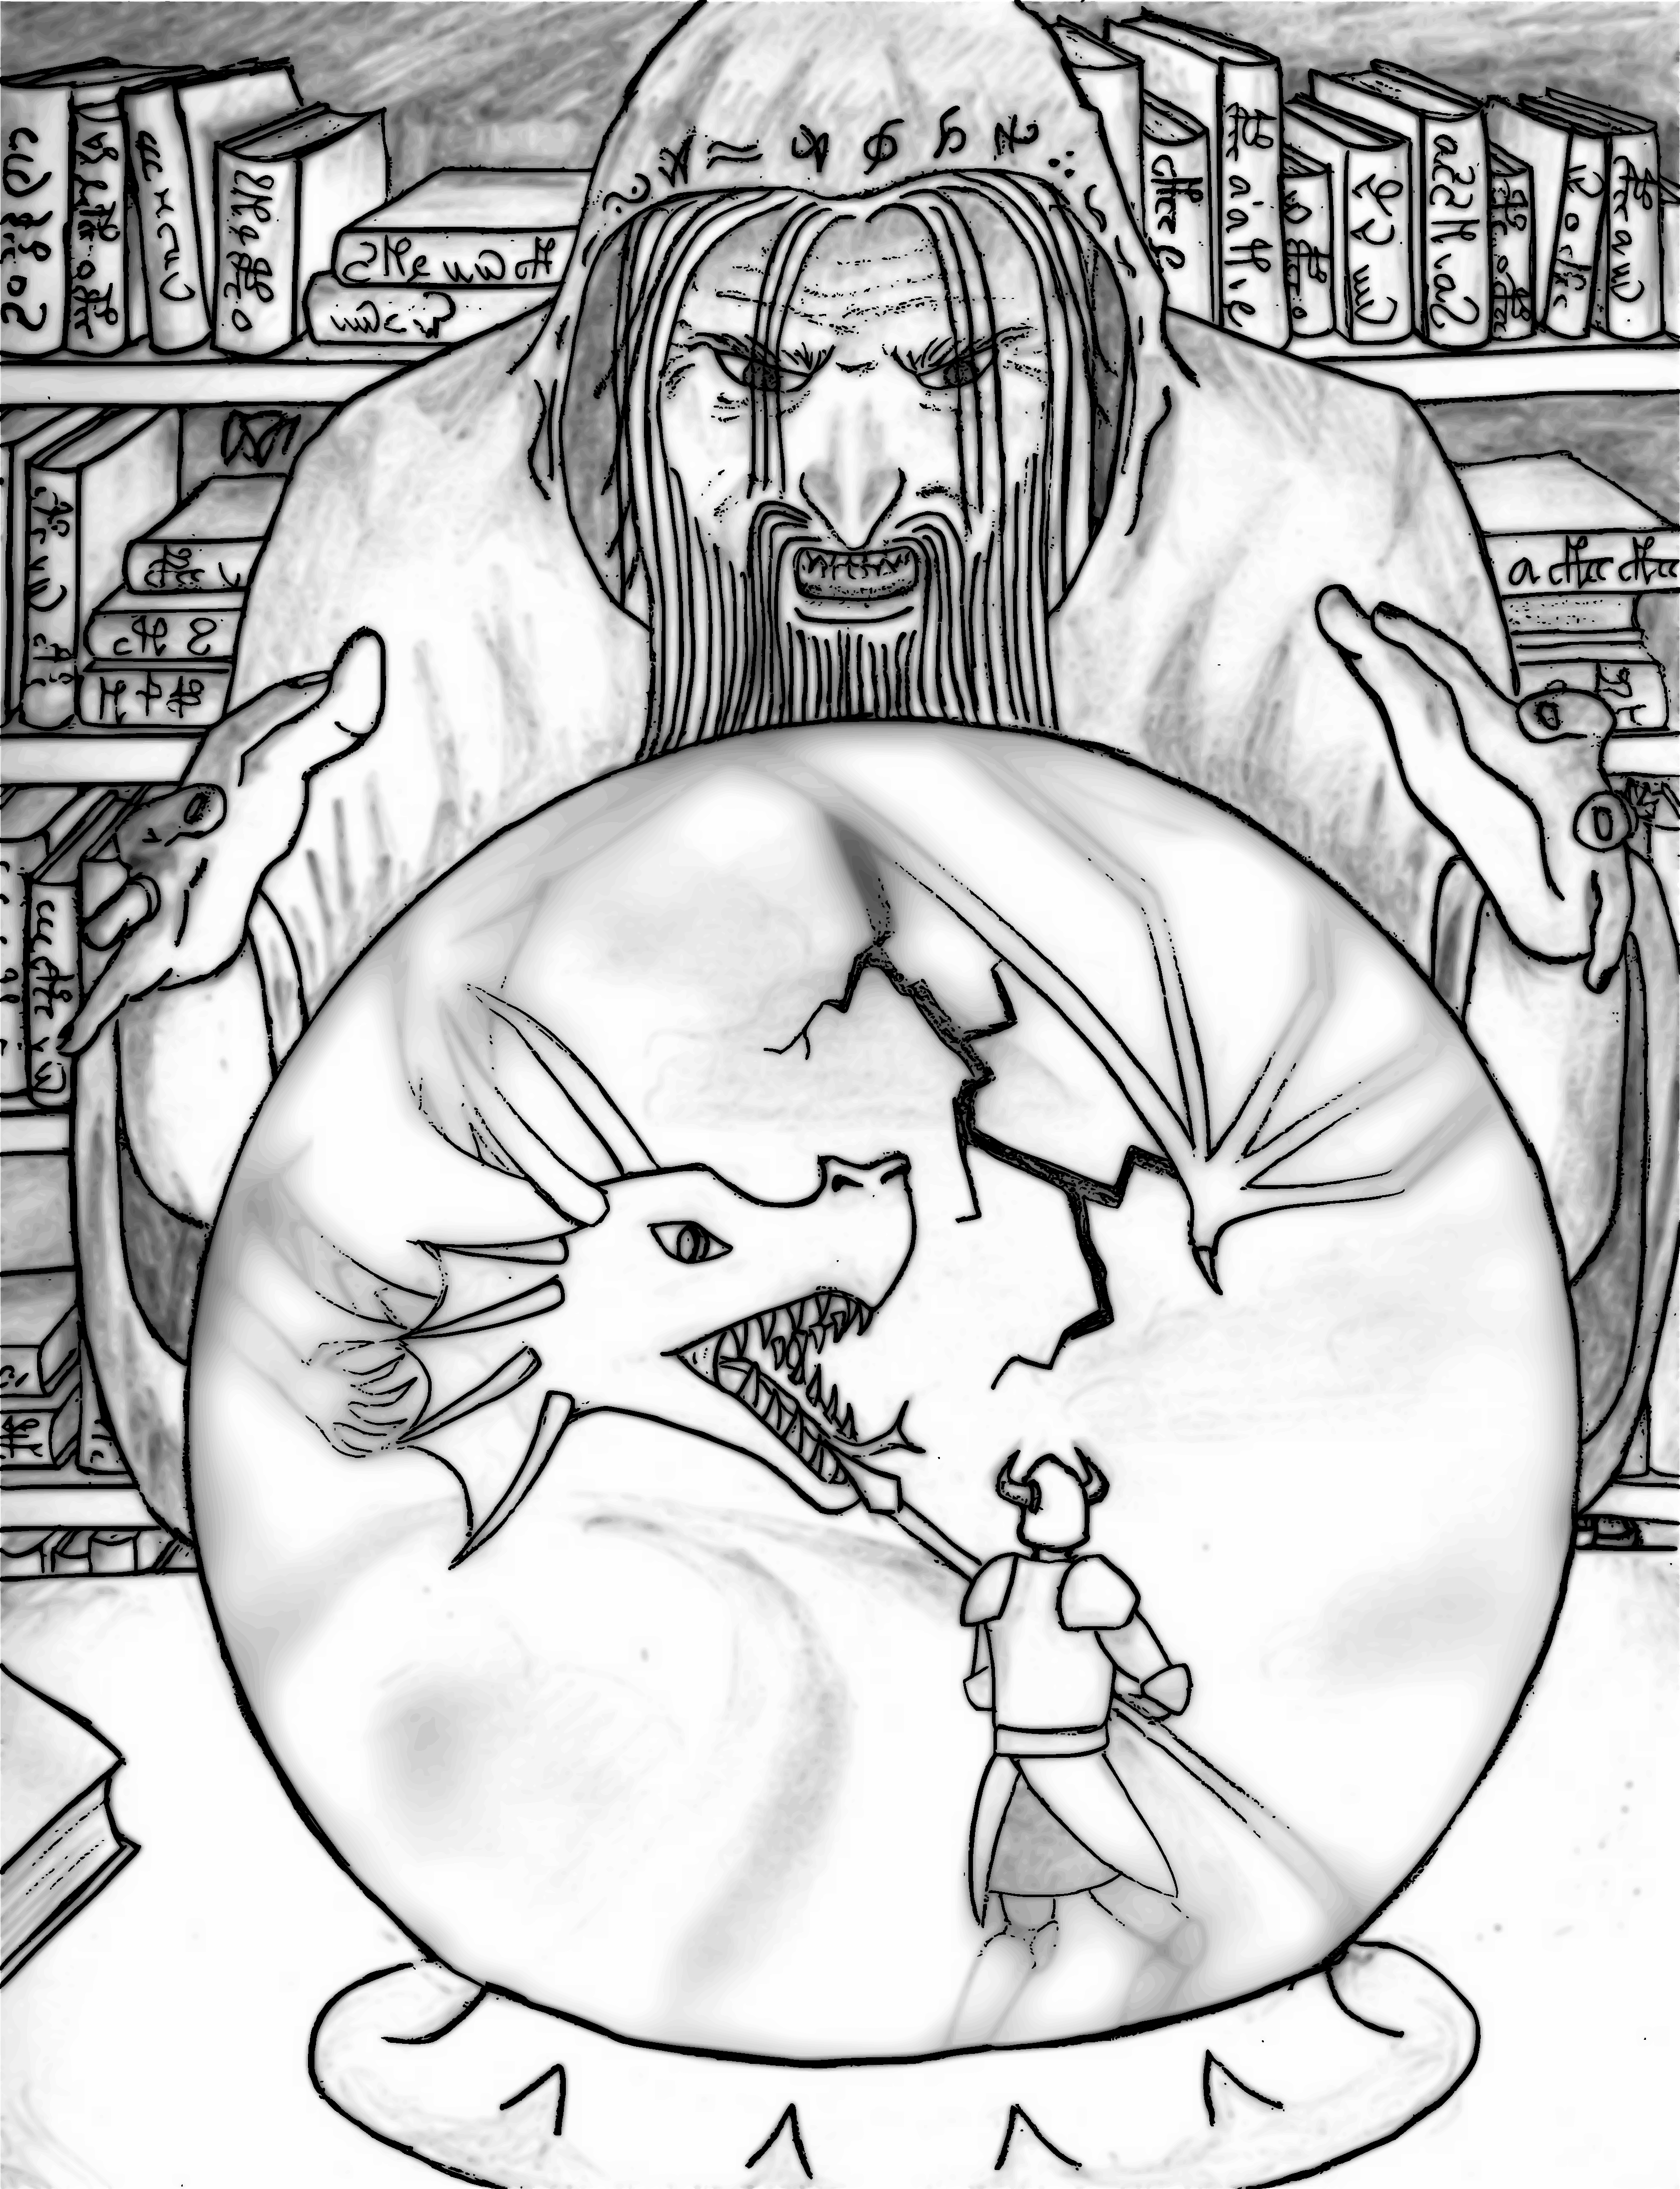
\includegraphics[width=\columnwidth]{staringthroughtheglass.pdf}\label{throughtheglass}
\pagebreak \thispagestyle{empty} \label{throughtheglass}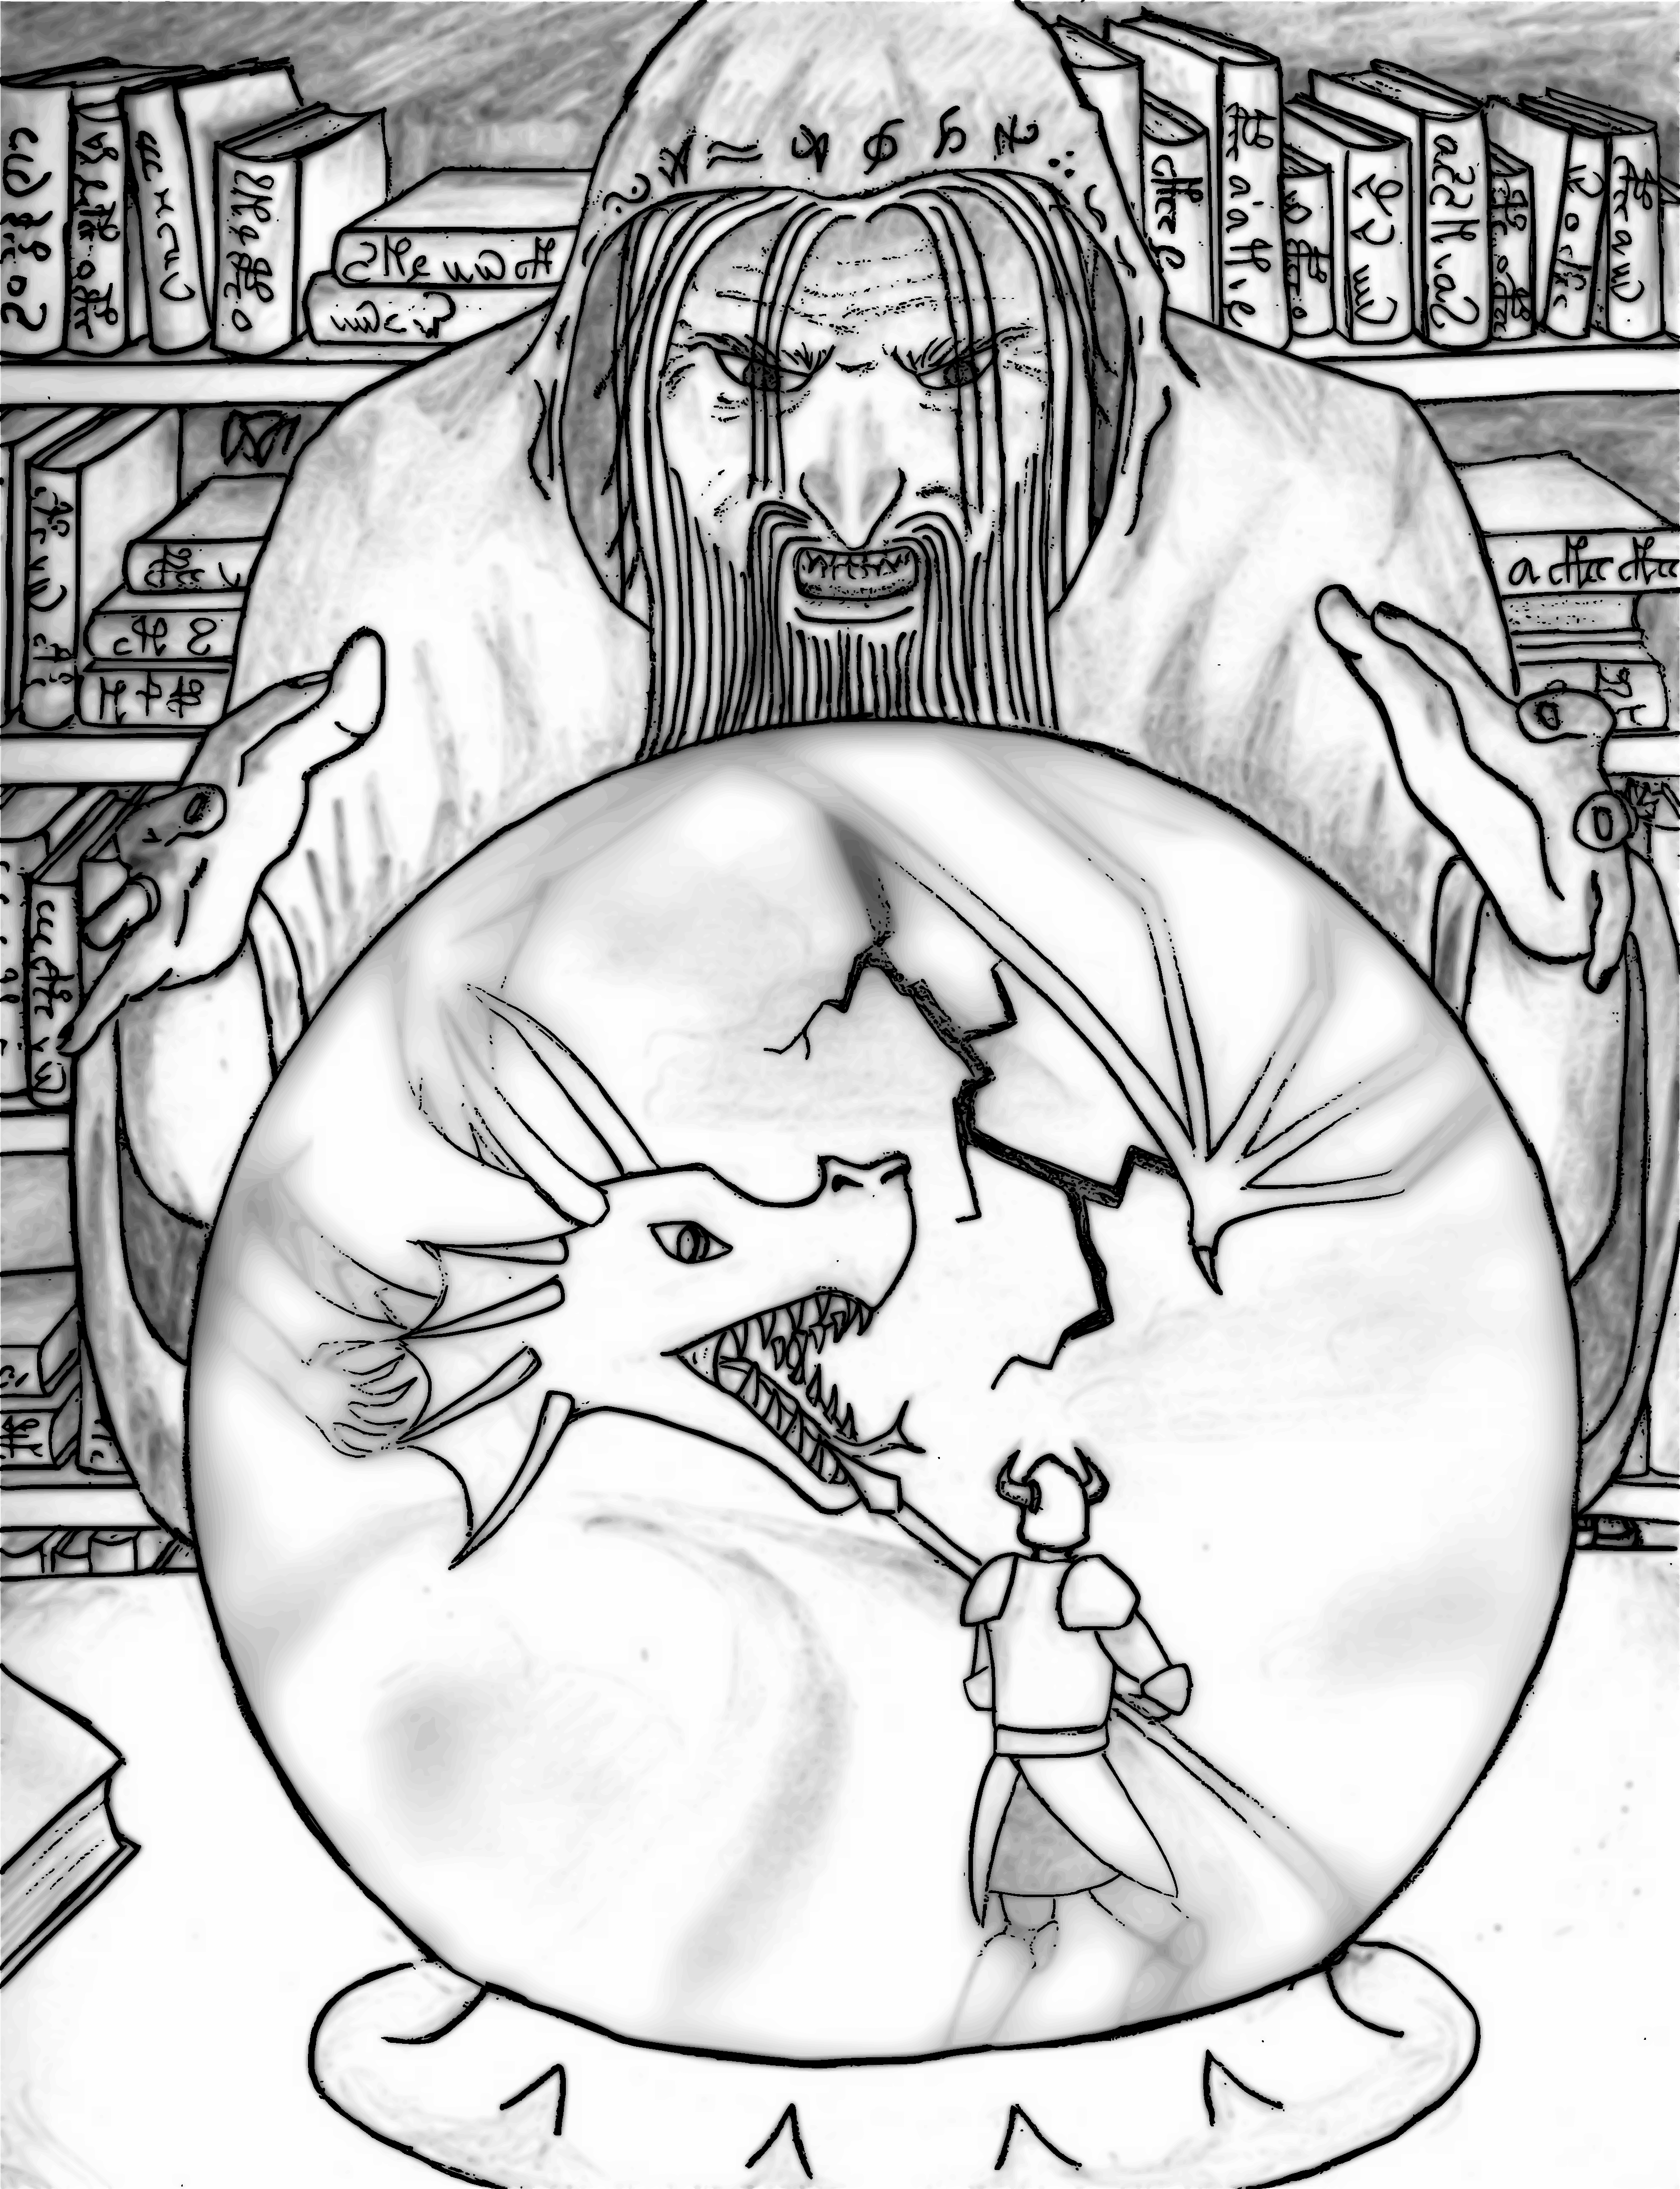
\includepdf[scale=1.007]{staringthroughtheglass.pdf}
